%Anna

% Domain layer 
% Data layer (firebase)
% tactics
%  - interfaces and listeners (dependecy injection) (composite pattern?)
%  - activity recognition vs significant
%  - No Location - new model for calculations
% choice of tecnhologies and sensors

\section{Application Architecture}



\section{Continuous Sensing Architecture}

The continuous sensing in this application is formed from the notions of:
\begin{itemize}
    \item Geofence 
    \item Location 
    \item Activity Recognition
\end{itemize}

When the user creates or applies to a bikebus two Geofences are created for the start and end destination on the route. When the user is within the one of the Geofences, the Geofence fires an event which either initiates or stops the data collection.
Concretely the application holds a SensorDataController, which controls the flow of sensor data. 
\begin{enumerate}
    \item Creating two Geofence pending intents from the GoogleGeofence class
    \item The GeofenceIntentService class receives a GoogleGeofenceEvent object when a Geofence is triggered
    \item Based on the information from the Geofence event the GeofenceIntentService sends a status and result value back to the SensorDataController through a BroadcastReceiver
    \item The SensorDataController either stops the activity recognition or creates pending intents at a given sample rate from the GoogleActivityRecognition class
    \item Each time the ActivityRecognizeService class receives an intent with a ActivityRecognitionResult object the intent service broadcasts the results back to the SensorDataController
    \item Based on the activity has the value "ON\_BICYCLE" the SensorDataController will retrieve the current location of the user and store all locations for data processing
\end{enumerate}

\begin{figure}[H]
\centering
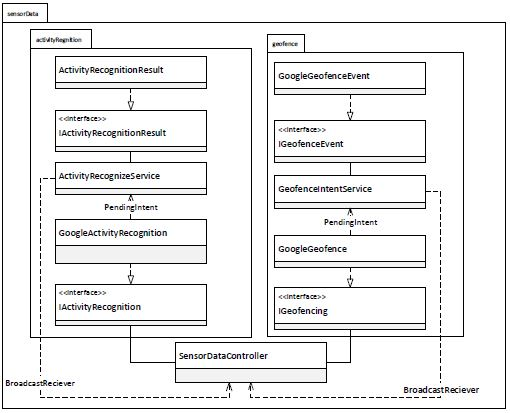
\includegraphics[scale=1]{Graphics/Images/Module_View_SensorData.jpg}
\caption{Module view of sensorData package}
\label{fig:Module_View_Sensor_Data}
\end{figure}
In figure \ref{fig:Module_View_Sensor_Data} a module view has been created based on the continuous data collection description. 

In Android there is typically two methods to apply when wanting to create background processes:
\begin{itemize}
    \item IntentService
    \item AsyncTask
\end{itemize}

The IntentService is a method used for long-term running background processes that is not dependent on the Activity. The AsyncTask is oppositely a method that only exists in the Activity's lifecycle, because it needs to return the value directly to the Activity. Therefore the AsyncTask cannot continue to run outside the application, and is more suited for short-term running background processes which are dependent on the Activity. 
\footnote{\url{https://github.com/codepath/android_guides/wiki/Starting-Background-Services}}

\section{Graphical User Interface}
The graphical design of this application is strongly inspired from another app called "GoMore", which has the concept of coordinating carpools. The "GoMore" concept reminds a lot about the "BikeBus" concept, because both apps coordinates for friends and strangers to ride with each other. The main differences between the two concepts are that "BikeBus" coordinates free bicycle rides and paid "GoMore" coordinates Car rides.

\begin{figure}
    \centering
    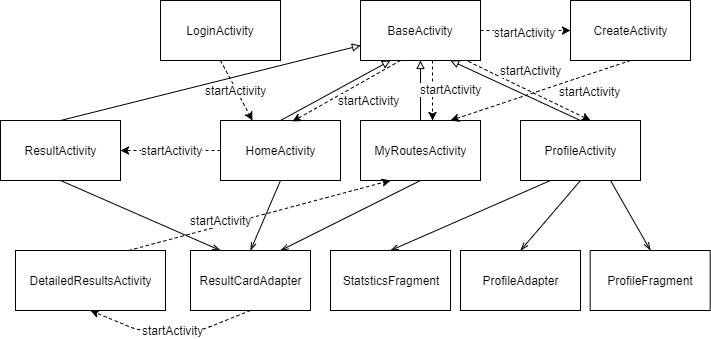
\includegraphics[scale=0.5]{Graphics/Images/Activity_Diagram.png}
    \caption{Diagram of activities}
    \label{fig:my_label}
\end{figure}

%% MISSING DESCRIPTION OF ACTIVITY DIAGRAM%%

\subsection{Design}
The "BikeBus" application follows the "Material Design" principles created by Google\footnote{\url{https://material.io/guidelines/#}}, which are quite popular for Android apps. Material Design has great guidelines on how to improve mobile user experience and can quickly make the application look more professional.

The Android GUI components used to provide the Material Design elements:
\begin{itemize}
    \item CardView - The card element containing information of the bikebus
    \item RecyclerView - Infinity scroll view containing only cardviews
    \item BottomNavigationView - The bottom navigation menu between search, routes and profile tabs
    \item TabLayout with ViewPager - A Tab view in the profile view which switches between the profile and statistics fragment
    \item FloatingActionButton - The red create button
\end{itemize}

In this project Google API's has been frequently used for especially sensor data, but the Google AutoComplete

\begin{figure}[!htb]
\centering
\begin{minipage}{0.32\textwidth}
\centering
    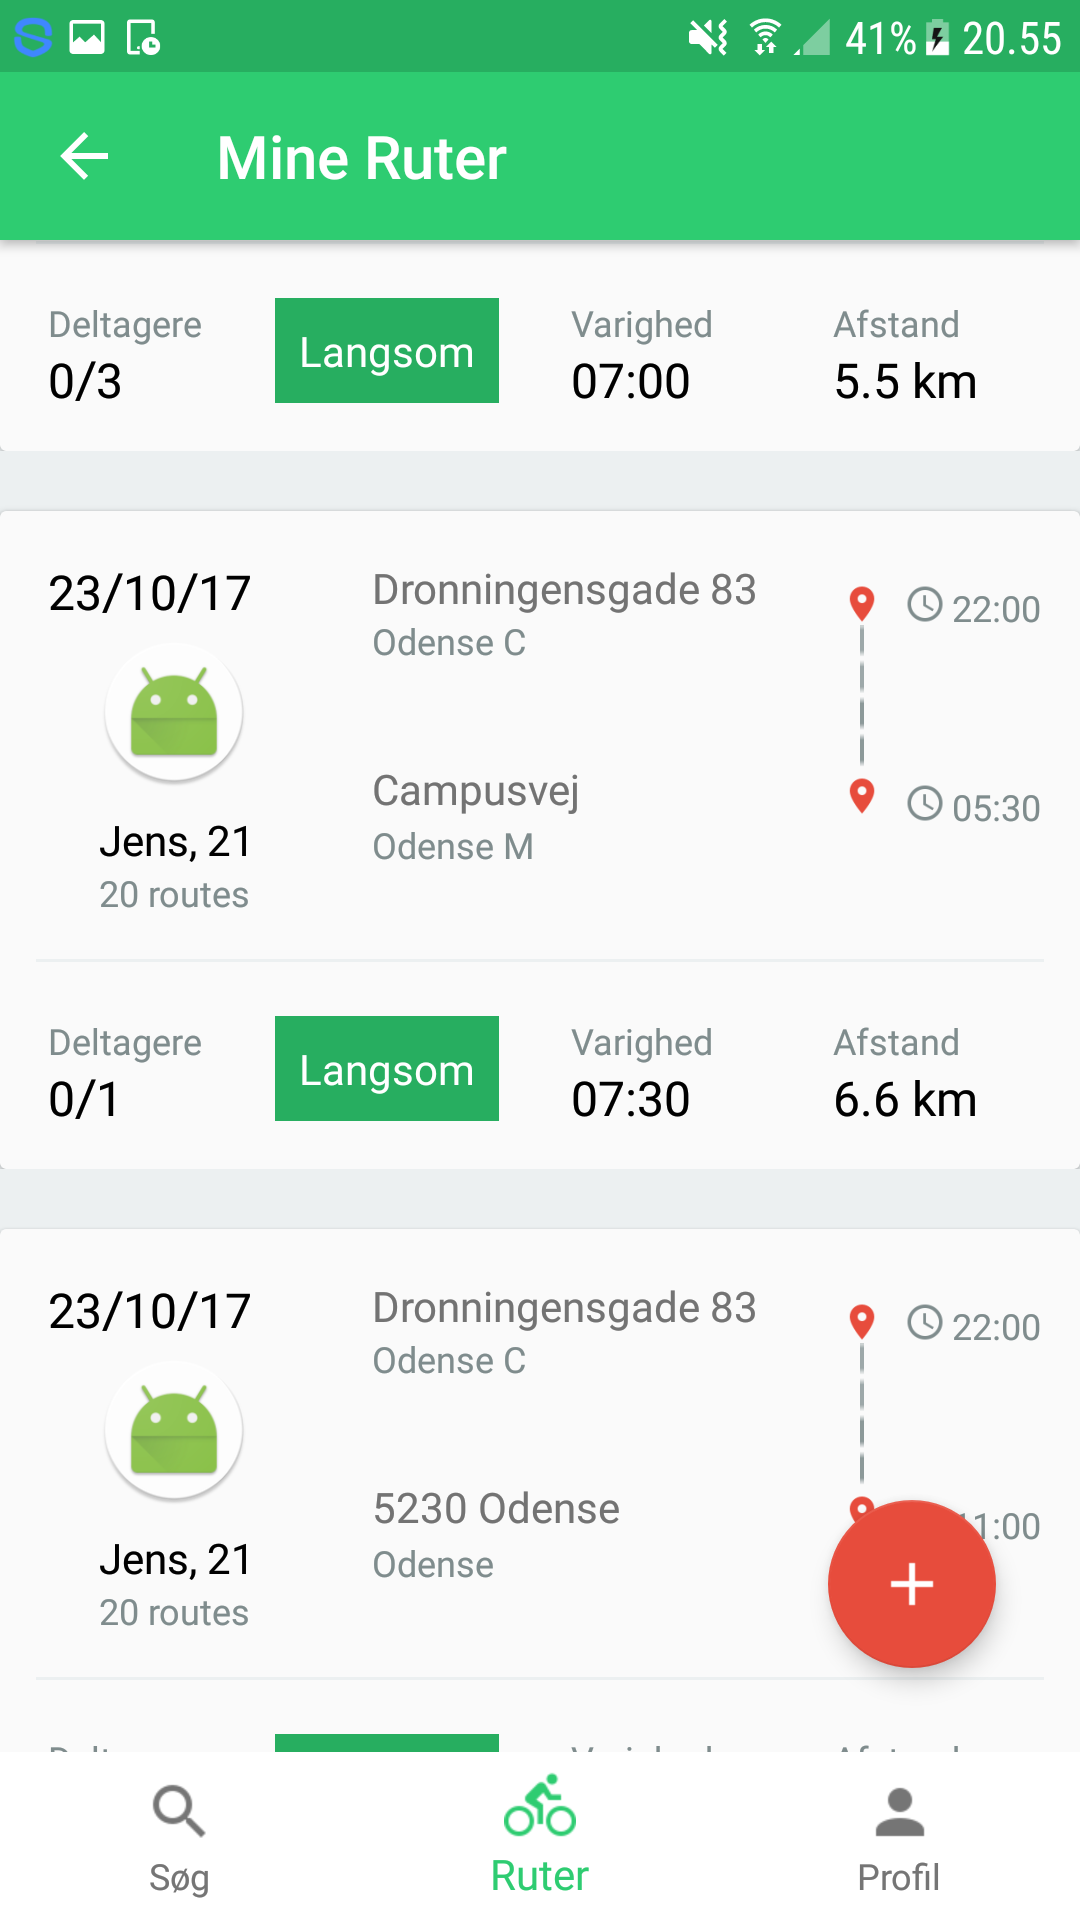
\includegraphics[width=\linewidth]{Graphics/Images/bikebus_search.png}
    \caption{Result page for BikeBus}
    \label{fig:sample_figure}
\end{minipage}\hfill
\begin{minipage}{0.32\textwidth}
\centering
    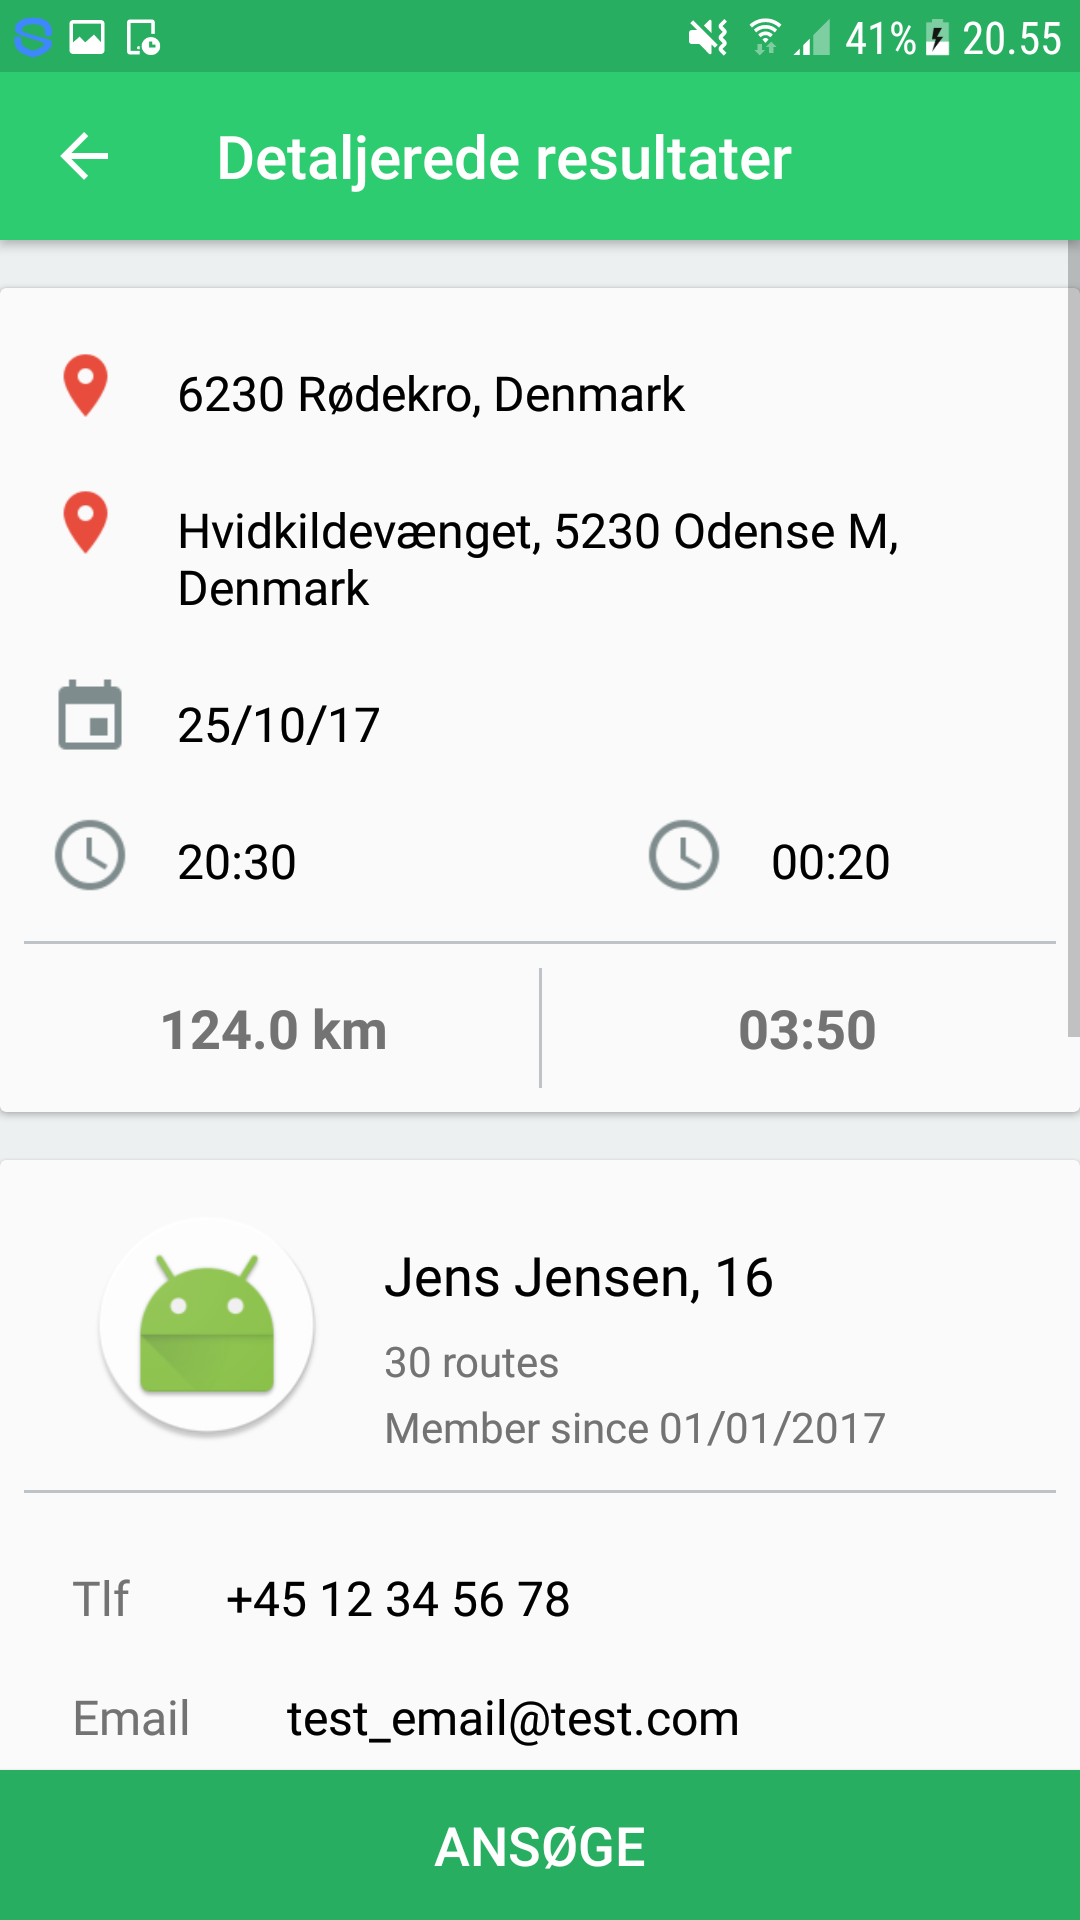
\includegraphics[width=\linewidth]{Graphics/Images/bikebus_detail_1.png}
    \caption{Detailed page for BikeBus (part 1)}
    \label{fig:sample_figure}
\end{minipage}\hfill
\begin{minipage}{0.32\textwidth}
\centering
    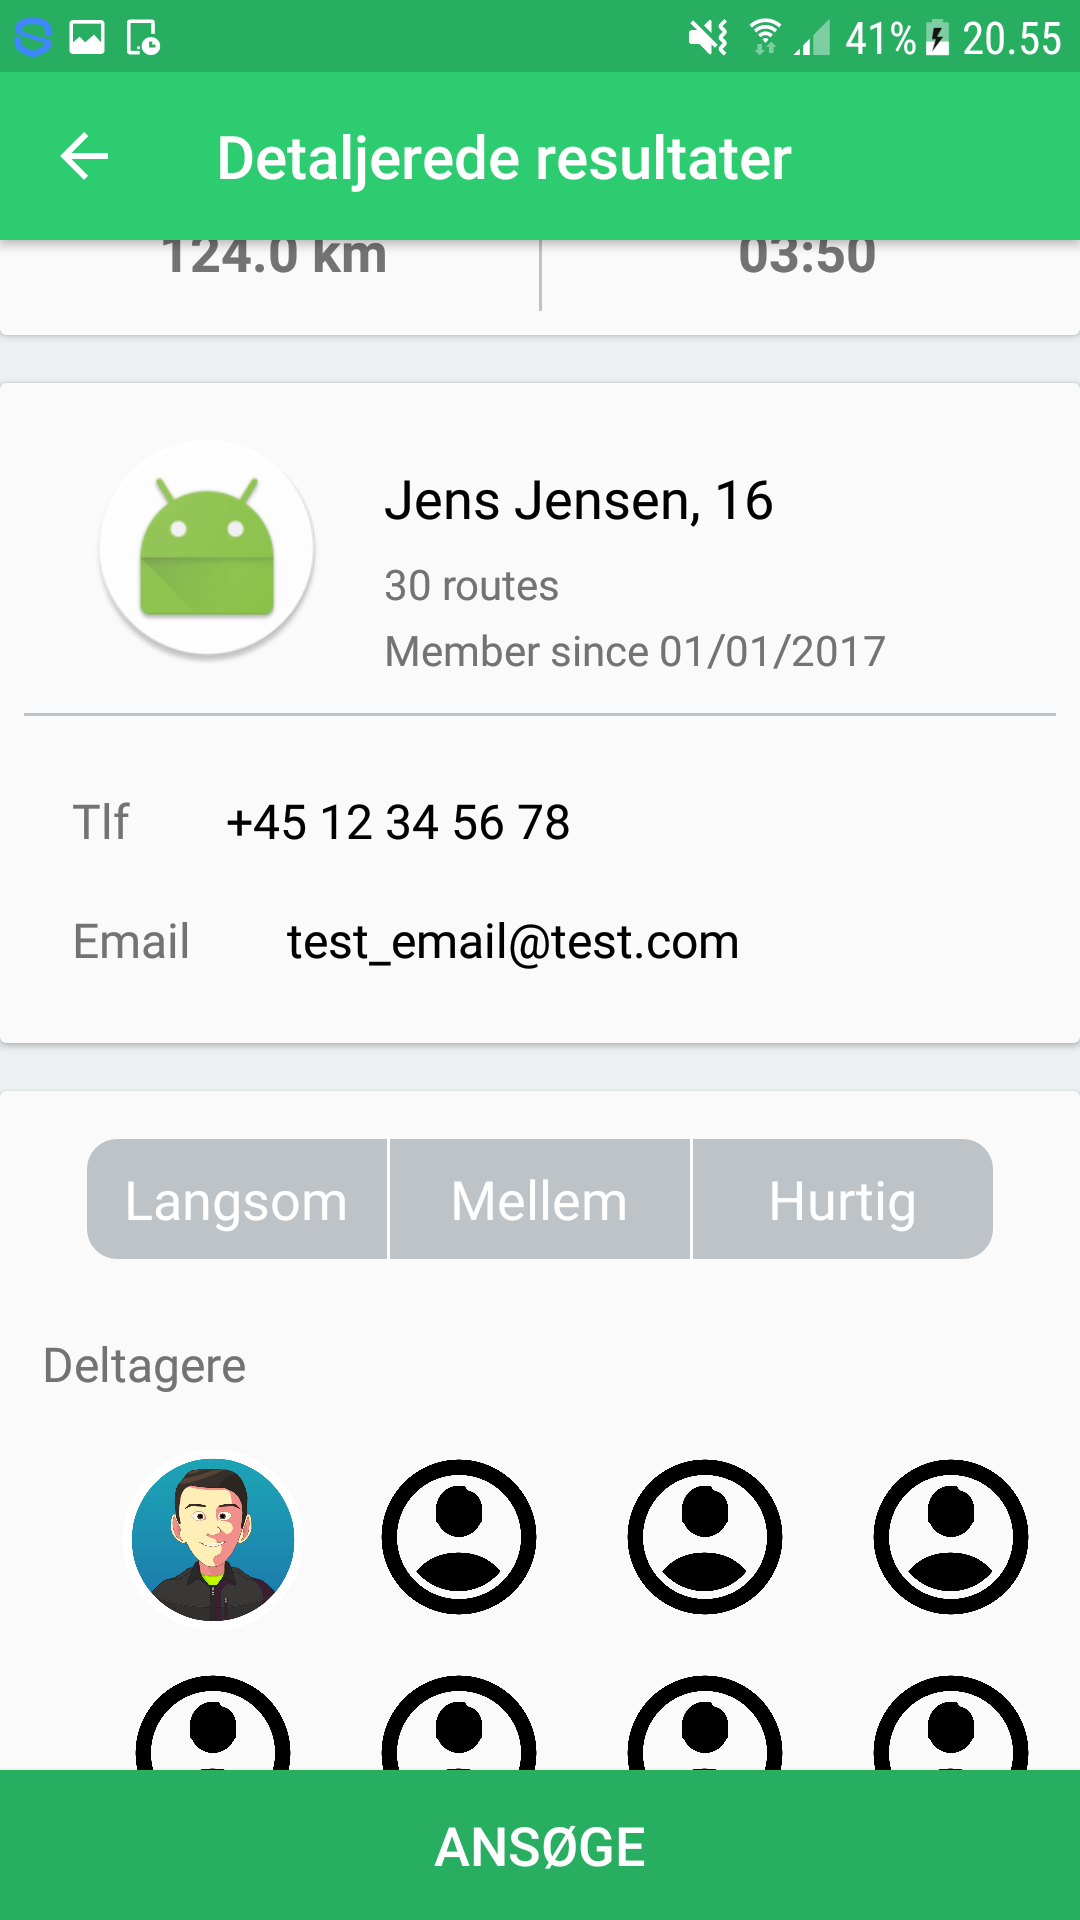
\includegraphics[width=\linewidth]{Graphics/Images/bikebus_detail_2.png}
    \caption{Detailed page for BikeBus (part 2)}
    \label{fig:sample_figure}
\end{minipage}
\end{figure}